% !TEX root = Eco-Model.tex
\section{Experiment and result Analysis} % (fold)
\label{sec:Experiment_results}

Because of the  autonomous and self-directed features of individuals in the manufacturing ecosystem, we use agent-based modeling and simulation(ABMS) technique \cite{Macal2009,north2007managing} to study such a complex system. Repast Simphony \cite{North2013} package was utilized in this experiment.

% \subsection{Agent-based modeling and simulation design} % (fold)
% \label{sub:agent_based_modeling_and_simulation}
% \subsubsection{Model realization}
% \begin{asparaenum}
% \item Main agents
% \suspend{asparaenum}
% \begin{figure}[htbp]
% \centering
% \tiny
% \subfloat[Job related classes]{\begin{tikzpicture}
%     % !TEX root = flow_head.tex

\begin{class}[text width=8cm]{Job}{0,0}
	\attribute{+ allocated: boolean}
	\attribute{+ allocation: Map}
	\attribute{+ candidates: Map}
	\attribute{+ inNeed: boolean}
	\attribute{+ needResourceCapacity: Map}
	\attribute{+ predecessor: Set}
	\attribute{+ prepareStatus: Map}
	\attribute{- processBehavior: ProcessBehavior}
	\attribute{- selectBehavior: SelectBehavior}
	\operation{+ addCandidates(competitor: Machine): void}
	\operation{+ CheckStatus(): void}
	\operation{+ Need(): void}
	\operation{+ Review(m: Machine): void}
	\operation{+ Select(watchedAgent: Job): void}
\end{class}


%     % !TEX root = flow_head.tex

\begin{class}[text width=8cm]{Task}{0,0}
	\attribute{+ master: Order}
	\attribute{+ owner: Map}
	\attribute{+ pause: boolean}
	\attribute{+ processingTime: int}
	\attribute{+ remainingTime: int}
	\attribute{+ type: Strihng}
	\operation{+ Task()}
	\operation{+ addOwner(user: User, p: int): void}
	\operation{+ CheckStatus(): void}
	\operation{+ Process(watchedAgent: Task): void}
	\operation{+ setParameters(taskData: Map): void}
\end{class}
%     % !TEX root = flow_head.tex

\begin{class}[text width=.225\textwidth]{ServiceCall}{1.08,-3.7}
	\inherit{Job}
	\attribute{+ owner: Provider}
	\attribute{+ type: String}
	\operation{+ ServiceCall()}
	\operation{+ setParameter(scData: Map): void}
	\operation{+ Recall(): void}
\end{class}
%     \end{tikzpicture}
%     \label{fig:jobclassed}}\hspace{1pt}
% \subfloat[Machine related classes]{\begin{tikzpicture}
%     % !TEX root = flow_head.tex

\begin{class}[text width=.45\textwidth]{Machine}{0,0}
	\attribute{+ assignBehavior: AssignBehavior}
	\attribute{+ buffer: List}
	\attribute{+ competeList: List}
	\attribute{+ jobList: List}
	\attribute{+ owner: Provider}
	\attribute{+ releaseBehavior: ReleaseBehavior}
	\attribute{+ responseBehavior: ResponseBehavior}
	\attribute{+ responseList: List}
	\attribute{+ type: String}
	\operation{+ Assign(t: Task): void}
	\operation{+ Release(j: Job): void}
	\operation{+ Reply(watchedAgent: Job): void}
	\operation{+ Response(watchedAgent: Task): void}
	\operation{+ Review(j: Job):void}
\end{class}


%     % !TEX root = flow_head.tex

\begin{class}[text width=.45\textwidth]{Resource}{-2.4,-3.66}
	\inherit{Machine}
	\attribute{+ available: int}
	\attribute{+ capacity: int}
	\attribute{+ master: Map}
	\attribute{+ needCap: Map}
	\attribute{+ sourceable: int}
	\operation{+ Resource()}
	\operation{+ addMaster(ser: Service, amonut: int): void}
	\operation{+ Assign(sc: ServiceCall, amount: int): void}
	\operation{+ Response(watchedAgent: ServiceCall): void}
\end{class}
%     % !TEX root = flow_head.tex

\begin{class}[text width=.45\textwidth]{Service}{2.4,-3.66}
	\inherit{Machine}
	\attribute{+ resourceComposition: Map}
	\operation{+ Service()}
	\operation{+ OutSource(): void}
\end{class}
%     \end{tikzpicture}
%     \label{fig:machineclassed}}\\
% \subfloat[User related classes]{\begin{tikzpicture}
%     % !TEX root = flow_head.tex

\begin{class}[text width=.45\textwidth]{User}{0,0}
	\attribute{- agentIDCounter: long}
	\attribute{\# agentID: String}
\end{class}
%     % !TEX root = flow_head.tex

\begin{class}[text width=.45\textwidth]{Provider}{-2.4,-1.2}
	\inherit{User}
	\attribute{+ candidates: List}
	\attribute{+ rank: double}
	\attribute{+ resourceList: List}
	\attribute{+ serviceList: List}
	\operation{+ GenerateResource(): void}
	\operation{+ GenerateService(serviceData: List): void}
	\operation{+ GenerateServiceCall(): void}
	\operation{+ RemoveServiceCall(sc: ServiceCall): void}
	
\end{class}
% % !TEX root = flow_head.tex

\begin{class}[text width=.45\textwidth]{Demander}{2.4,-1.2}
	\inherit{User}
	\attribute{+ orderList: List}
	\attribute{+ taskMap: Map}
	\operation{+ GenerateOrder(orderID: String): void}
	\operation{+ ReadData(orderID: String): void}
\end{class}


%     \end{tikzpicture}\label{fig:userclassed}}\hspace{3pt}
% \subfloat[Cloud Platform]{\begin{tikzpicture}
% 	% !TEX root = flow_head.tex

\begin{class}[text width=8cm]{CloudPlatform}{0,0}
	\attribute{- agentIDCounter: long}
	\attribute{\# agentID: String}
	\attribute{+ finishCount: int}
	\attribute{+ userList: List}
	\operation{+ CreateProvider(): void}
	\operation{+ CreateDemander(): void}
\end{class}


% 	\end{tikzpicture}\label{fig:platform}}
% \end{figure}


% \resume{asparaenum}
% \item Behavior interfaces and classes
% \end{asparaenum}

% \begin{figure}[htbp]
%     \centering
%     \tiny
%     \begin{tikzpicture}
%     % !TEX root = flow_head.tex

\begin{interface}[text width=.45\textwidth]{AssignBehavior}{0,0}
	\operation{+ BufferEnterance(t: Task, m: Machine): boolean}
	\operation{+ Queue(j: Job, m: Machine): void}
	\operation{+ Buff(t: Task, m: Machine): void}
\end{interface}


%     % !TEX root = flow_head.tex

\begin{interface}[text width=.45\textwidth]{SelectBehavior}{0,-1.7}
	\operation{+ Allocate(theOnes: Map): Map}
	\operation{+ Assign(allocation: Map, j: Job): void}
	\operation{+ Evaluation(j: Job, candidates: List): void}
	\operation{+ Select(j: Job, candidates: List): void}
\end{interface}
%     % !TEX root = flow_head.tex

\begin{interface}[text width=.45\textwidth]{ResponseBehavior}{0,0}
	\operation{+ Exist(j: Job, m: Machine): boolean}
\end{interface}
%     % !TEX root = flow_head.tex

\begin{interface}[text width=.45\textwidth]{ProcessBehavior}{4.8,-2.35}
	\operation{+ Process(j: Job): void}
\end{interface}
%     % !TEX root = flow_head.tex

\begin{interface}[text width=8cm]{ReleaseBehavior}{0,0}
	\operation{+ Release(j: Job, m: Machine): void}
	\operation{+ Next(m: Machine): void}
\end{interface}
%     % % !TEX root = flow_head.tex

\begin{class}[text width=8cm]{ServiceAssign}{0,0}
	\operation{+ BufferEnterance(t: Task, m: Machine): boolean}
	\operation{+ Queue(j: Job, m: Machine): void}
	\operation{+ Buff(t: Task, m: Machine): void}
\end{class}
%     % % !TEX root = flow_head.tex

\begin{class}[text width=.45\textwidth]{ResourceAssign}{2.4,-2.5}
	\implement{AssignBehavior}
	\operation{+ Buff(t: Task, m: Machine): void}
	\operation{+ BufferEnterance(t: Task, m: Machine): boolean}
	\operation{+ Queue(j: Job, m: Machine): void}
\end{class}
%     \end{tikzpicture}
%     \caption{Assign interface and related classes}
%     \label{fig:assigninterface}
% \end{figure}


\subsection{Experiments} % (fold)
\label{ssub:case_design}
We design experiments to repeatedly simulate the operating of ecosystem from the very beginning with mode combinations in \autoref{tab:grouping} group by group, which are the prototypes of feasible cloud manufacturing operating modes. Every single simulation goes with the main flow as show in \autoref{fig:originmode}. We use  RanGen \cite{Demeulemeester2003} to generate dataset in the well-known Patterson format as the the continuously arriving order for the simulation input, related parameter settings are listed in \autoref{tab:generalparameter}.
\begin{table}[htbp]
  \centering
  \scriptsize
  \caption{Order generating parameters setting}
    \begin{tabular}{cccccccccc}
    \toprule
    \textbf{$n_a$} & \textbf{OS} & \textbf{CI} & \textbf{$n_r$} & \textbf{RF} & \textbf{RC} & \textbf{$\lambda_d$} &\textbf{$\lambda_p$} & \textbf{$C_{k,0}$}\\
    \midrule
     10  &   0.3    &  [2,3]     &   12     &  0.3     &   0.5  & 0.2 & 0.3  & [20,30] \\
    \bottomrule
    \end{tabular}%
    {\footnotetext{\tiny The meaning of the first 5 parameters are defined in \cite{Demeulemeester2003}, $\lambda$ is the parameters of the arrival of user in simulation, $C_{k,0}$ is the initial capacity for $mr_k$}
    }
  \label{tab:generalparameter}%
\end{table}%

We assume that providers and demanders are arriving as the Poisson process, in order to make sure the coming need resource capacity rate will not exceed the average coming resource capacity rate in average to prevent the task explosion, and we make sure that,
\begin{equation}
\lambda_d n_a n_r \cdot RF \cdot RC < \lambda_p \bar C_{k,0} \label{eq:balance}
\end{equation}


\begin{table}[htbp]
  \centering
  \scriptsize
  \caption{Experiments mode grouping}
    \begin{tabular}{llcc}
    \toprule
          &       & Without metabolism & With metabolism \\
    \midrule
    \multicolumn{2}{l}{Resource-only} & Mode 11 & Mode 12 \\\hline
    \multicolumn{1}{l}{\multirow{2}[0]{*}{Service-incubate}} & without outsource & Mode 21 &Mode 22 \\\cline{2-4}
    \multicolumn{1}{l}{} & with outsource & Mode 31 & Mode 32 \\
    \bottomrule
    \end{tabular}%
  \label{tab:grouping}%
\end{table}%
% subsubsection parameters_setting (end)

\subsection{Result and analysis} % (fold)
\label{ssub:result_and_analysis}
Experiment on each mode in one group are simulated with same random seed to make no difference on the coming of order, provider and other irrelevant configuration to our validation.  After bunch of experiments with different random seeds, take random seed 776189616 as example, we run the simulation for 6000 tick time and the experiment's results are displayed in \autoref{fig:out} and \autoref{tab:averagevalue}, meaning of new most symbols are defined as the title of all the plots in \autoref{fig:out}, $RE$ denotes the resource efficiency determined by \autoref{eq:re}
\begin{equation}
  RE = \frac{\bar N_F}{\bar N_R} \label{eq:re}
\end{equation}
\begin{table}[htbp]
    \caption{Average observed values}
    \label{tab:averagevalue}
    \centering
    \scriptsize
    \begin{tabular}{lcccccc}
    \toprule
    \textbf{Mode} & $\bar N_T$ & $\bar N_F$ & $\bar N_P$ & $\bar N_R $ & $\bar Q$ & $RE$\\
    \midrule
    Mode 11 & 1159.360 &  1644.201 &  1177.601 &  2053.727 &  8.388 & 0.801\\
    Mode 21 & \textit{636.769} &  \textit{2031.215} &  \textbf{692.716} &  \textbf{1066.947} &  16.016 & 1.904\\
    Mode 31 & 779.413 &  1996.021 &  \textit{782.272} &  \textit{1203.748} &  15.174 & 1.658\\
    Mode 12 & 1439.831 &  1522.923 &  1797.883 &  2954.113 &  14.057 & 0.516\\
    Mode 22 & \textbf{343.444} &  \textbf{2464.407} &  1316.952 &  1957.226 &  \textit{20.251} & 1.259\\
    Mode 32 & 1164.409 &  1907.011 &  1597.742 &  2428.155 &  \textbf{20.652} & 0.785\\

    \bottomrule
    \end{tabular}
\end{table}
we find: \begin{asparaenum}[1)]
\item Most dotted lines are above the full lines with the same series in $N_R,N_P,N_T$ means that metabolism mode need lower number of provider and resource, with the price of higher number of queue length of the tasks in resources in the system to deal with the same amount of needs, except for Mode 22. Full lines are not much above dotted lines in $N_F$ means that task finish rate will be a little lower with the metabolism, exception also appears in Mode 22.
\item $L$ and $N_T$ both represent the job queue length, triangle and square line turned lower in $L$ means that incubation mode can help reduce the waiting of job, these two type of line above the circle line means the incubation mode do reduce the resource idle rate.
\item Triangle lines are a little above the square lines in $N_R,N_P,N_T$ means that outsourcing mode needs more resources to operate and can only reduce the job queue length a little.
\item There is no big difference among all the 6 modes in rank change. Provider in metabolism mode will get lower rank value for they cannot stay in the system for a longer time to get higher rank value. Provider in Mode 11 even will not promote their rank value, which means that the metabolism rate is very fast if without incubation mode.
\item Mode 22 is a very special mode that reached the balance within 6000 ticks, that the number of provider and resource changes little with time goes by. Because our experiment setting comply \autoref{eq:balance}, the coming need capacity rate is lower than the coming capacity rate, Mode 12,22,32 will finally reach balance in the long run theoretically, but the appearance of service-call and metabolism mode itself is full of uncertainty, thus it's hard to predict when other metabolism related mode will reach the balance.
\item With the average data value shown in \autoref{tab:averagevalue}, metabolism with incubation but not with outsourcing mode is one ideal combine mode to maintain the system, resource will self-configured and controlled to justly meet the task need.
\end{asparaenum}
\begin{figure}[htbp]
    \centering
    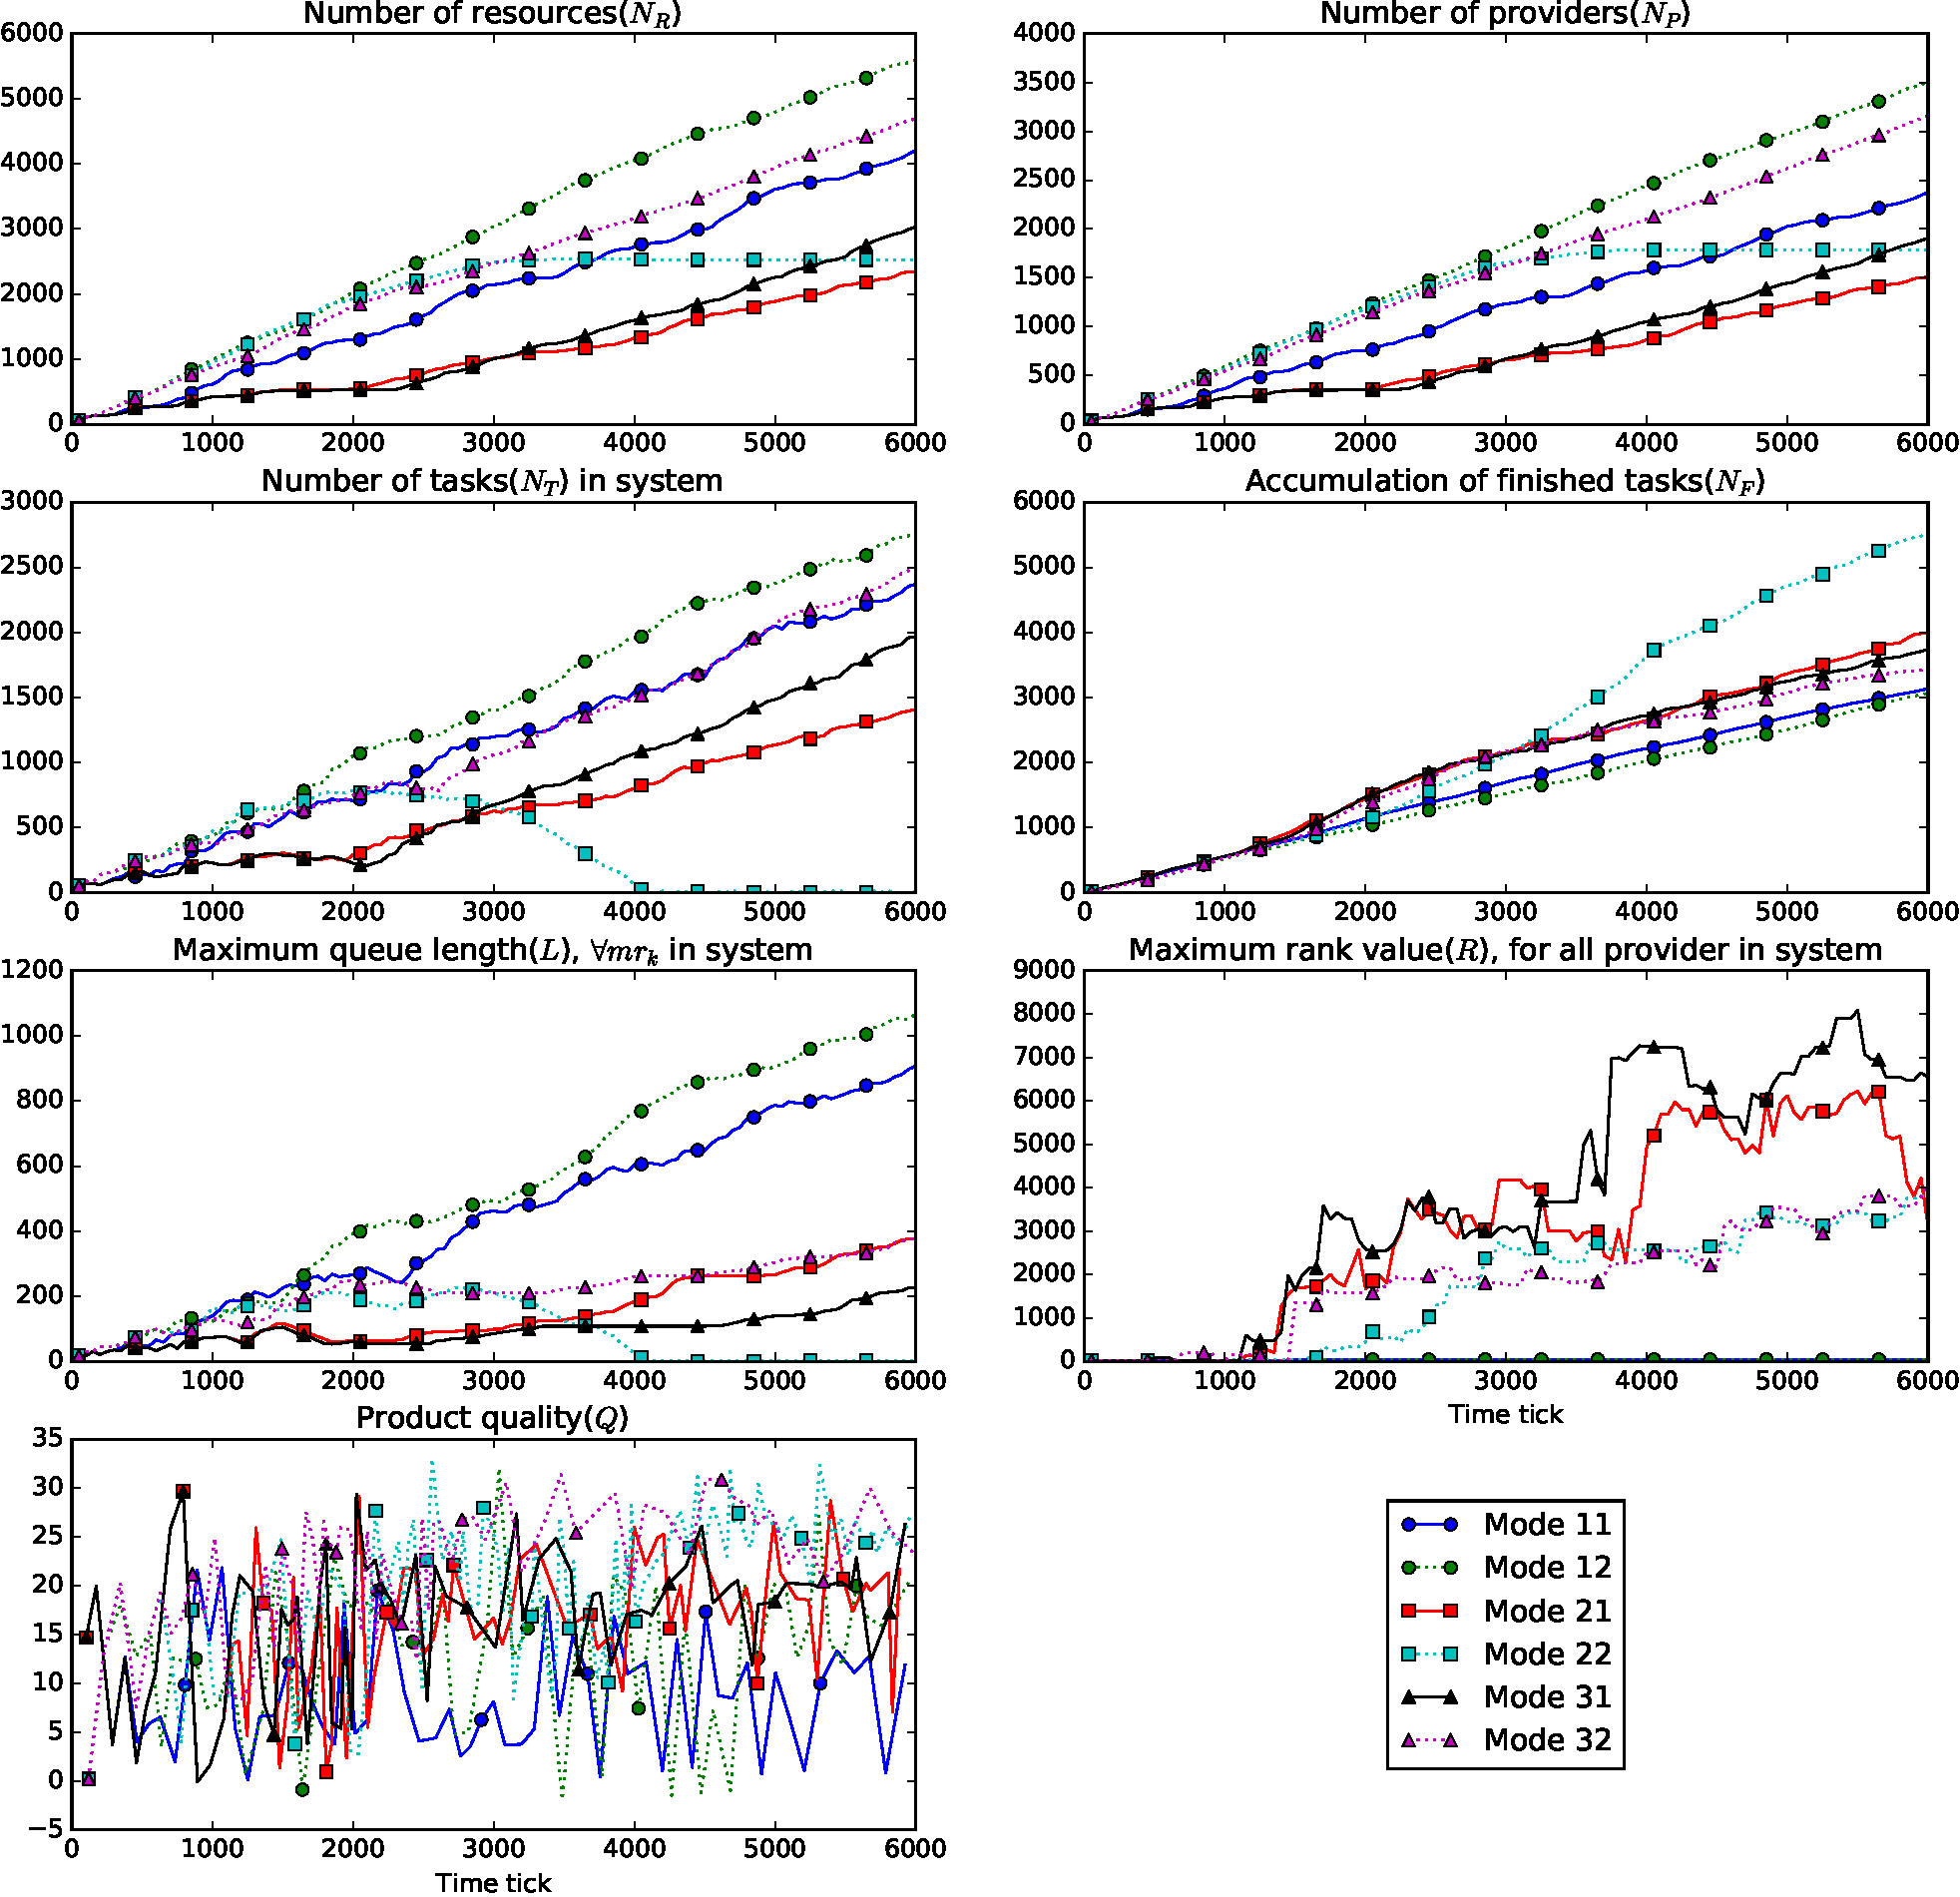
\includegraphics[width=\textwidth]{figures/out_new.pdf}
    \caption{Observed variable change with time}
    \label{fig:out}
\end{figure}
% subsubsection result_and_analysis (end)
